\section{Sphinx Packet Format}

HOPR uses the SPHINX packet format to encapsulate and route data packets in order to provide privacy features such as sender and receiver unlinkability.
Sphinx is a cryptographic message format used to relay anonymized messages within a mix network. A sphinx packet consists of two parts:

\begin{enumerate}
\item Header:
\begin{itemize}
\item Key derivation
\item Routing information
\item Integrity protection
\end{itemize}
\item Body:
\begin{itemize}
\item Onion-Encrypted payload
\end{itemize}
\end{enumerate}
\begin{figure}[H]
    \centering
    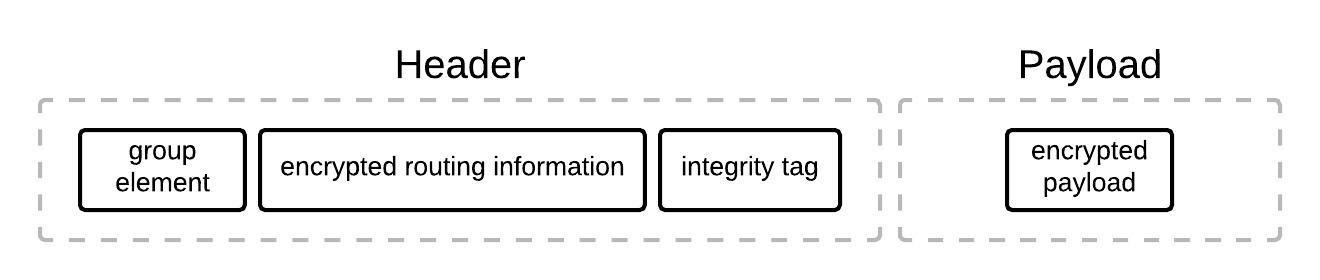
\includegraphics[width=11cm,height=11cm,keepaspectratio]{../whitepaper/images/sphinx.jpeg}
    \caption{Sphinx packet format}
    \label{fig:Sphinx packet format}
\end{figure}
\paragraph{Key derivation}
The sender (A) picks a random $x\in \mathbb{Z}^*_q$ that is used to derive new keys for every packet. 
\newline (A) randomly picks a path consisting of intermediate nodes (B), (C),(D) [see section path-finding] and the final destination of the packet (Z) 
\newline (A) performs an offline Diffie-Hellman key exchange with each of these nodes and derives shared keys with each of these nodes.
\newline (A) computes a sequence of $r$ tuples (in our case r=4)  $$(a_0,s_0,b_0),.................,(a_{r-1},s_{r-1},b_{r-1})$$ as follows:
\begin{itemize}
\item $a_0=g^x,s_0=y^x_B,b_0=h(a_0,s_0)$
\item $a_1=g^{xb_0},s_1=y^{xb_0}_C,b_1=h(a_1,s_1)$
\item $a_2=g^{xb_0b_1},s_2=y^{xb_0b_1}_D,b_2=h(a_2,s_2)$
\item $a_3=g^{xb_0b_1b_2},s_3=y^{xb_0b_1b_2}_D,b_3=h(a_3,s_3)$
\end{itemize}
 Where $y_B,y_C,y_D,y_Z$ are the public keys of the nodes $B,C, D$  which we assume to be available to $A$ . The $a_i$ are the group elements which, when combined with the nodes’ public keys, allows computing a shared key for each via Diffie-Hellman (DH) key exchange, 
 and so the first node in the user-chosen route can forward the packet to the next, and only that mix-node can decrypt it.
The element $g$ is a generator of $G$ which is a prime order cyclic group satisfying the Decisional DH Assumption. The used cyclic group in the HOPR Sphinx implementation is an elliptic curve group on the Ethereum secp256k1 curve and thus operations will be done on the elliptic curve. The $s_i$ are the DH shared secrets, $b_i$ are the blinding factors and $h$ is a hash function which is used to compute blinding factors.



\paragraph{Routing information}
Each node on the path needs to know the next downstream node. Therefore, the sender $(A)$ generates routing information $\beta_i$ for $(B)$, $(C)$ and (D) as well as message END to tell $(Z)$ that it is the final receiver of the message. 
\newline As $(A)$ has a shared secret with each of the nodes along the path, it is able to derive blindings for each of them.
\newline Once $(B)$ receives the packet, it derives the shared key $s_0$ by computing $$s_0=(a_0)^b=(g^x)^b=(g^b)^x=y^x_B$$ and removes its blindings. This allows $(B)$ to unblind the routing info that tells $(B)$ the public key of the next downstream node $(C)$ and deletes the routing information from the header. Afterwards, it fills the empty space with its own blinding.
\\$(B)$ also removes one layer of encryption from the payload.
Same happens at $(C)$ and $(D)$: key derivation, unblinding, deleting, shifting, decryption and blinding. 
In addition to all these steps, the final mix-header to the destination node $(Z)$ must include a final destination address that symbolizes the end of the path and tells that it’s the recipient and an Identifier used to generate reply messages back to the sender.
\\~\\Some padding is added at each mix stage, in order to keep the length of the message invariant at each hop. In the original Sphinx paper, a zero-byte padding is added which could reveal information about the path length and the final destination and thus breaking the SPHINX security properties.

\paragraph{Integrity}
Each node along the path receives an authentication tag $\gamma_i$ in the form of a message authentication code (MAC)
which is encoded in the header. In HOPR, we use a MAC based on a hash function BLAKE2s which is a cryptographic hash function faster than SHA-2 and SHA-3, yet is at least as secure as SHA-3 and produces digests of any size between 1 and 32 bytes. 
\\By using the derived shared secret $s_i$, each node is able to recompute the authentication tag and check the integrity of the received packet as follows: $$\gamma_i=HMAC(s_i,\beta_i)$$
This integrity check allows to verify whether or not the header was modified.

\paragraph{Encrypt \& Decrypt}
The payload is where the actual message is hidden and is computed in different layers using a block cipher encryption algorithm and is decrypted at each stage of mixing. LIONESS implementation based on the ChaCha20 stream cipher and the BLAKE2 hash algorithm is being used for encryption and decryption of the payload in HOPR's implementation of the SPHINX packet format. Any attempt of modification by an attacker would result in message distruction and thus is would be irrecoverable. 









